\documentclass[12pt,addpoints]{evalua}
\grado{3$^\circ$ de Secundaria}
\cicloescolar{2023-2024}
\materia{Matemáticas 3}
\unidad{2}
\title{Examen de la Unidad}
\aprendizajes{
      \item Resuelve problemas mediante la formulación y solución algebraica de ecuaciones lineales.
      \item Calcula el perímetro de polígonos y del círculo, y áreas de triángulos y cuadriláteros desarrollando y aplicando fórmulas.
      \item Calcula el volumen de prismas y cilindros rectos.
      }
\author{Prof.: Julio César Melchor Pinto}
\begin{document}
\begin{questions}
      \question[10]{Determina las medidas de tendencia central en los siguientes conjuntos de datos. \textit{(De ser necesario redondea tu respuesta a la decima más cercana)}:
            \begin{multicols}{2}
                  \begin{parts}
                        \part 80, 86, 85, 88, 80, 88, 81, 85, 95, 88, 88, 87, 100. \\[1em]
                        La media es: \fillin[$87$][0in]

                        \begin{solutionbox}{1cm}
                        \end{solutionbox}

                        La mediana es: \fillin[$87$][0in]

                        \begin{solutionbox}{1cm}
                        \end{solutionbox}

                        La moda es: \fillin[$88$][0in]

                        \begin{solutionbox}{1cm}
                        \end{solutionbox}

                        La desviación media es: \fillin[$3.8$][0in]

                        \begin{solutionbox}{2cm}
                        \end{solutionbox}

                        \columnbreak%

                        \part 26, 22, 25, 24, 28, 29, 22, 24, 22, 27, 26. \\[1em]
                        La media es: \fillin[$25$][0in]

                        \begin{solutionbox}{1cm}
                        \end{solutionbox}

                        La mediana es: \fillin[$25$][0in]

                        \begin{solutionbox}{1cm}
                        \end{solutionbox}

                        La moda es: \fillin[$22$][0in]

                        \begin{solutionbox}{1cm}
                        \end{solutionbox}

                        La desviación media es: \fillin[$2.6$][0in]

                        \begin{solutionbox}{2cm}
                        \end{solutionbox}
                  \end{parts}
            \end{multicols}
      }


      % \subsection*{Eventos mutuamente excluyentes}
      \question[8]{Resuelve los siguientes problemas:

            \begin{parts}
                  \part Si se lanzan tres monedas al aire, calcula la probabilidad de que caiga puro sol.

                  \begin{solutionbox}{1.5cm}
                  \end{solutionbox}

                  \part Calcula la altura de un prisma que tiene como área de la base 8 m$^2$ y 120 m$^3$ de capacidad.

                  \begin{solutionbox}{1.5cm}
                  \end{solutionbox}

                  % \part Ricardo quiere poner una barda alrededor de un terreno pentagonal que mide 15 metros por lado. ¿Cuánta barda necesitará Ricardo para poner barda en todo el terreno?

                  % \begin{solutionbox}{1.2cm}
                  % \end{solutionbox}


            \end{parts}
      }

      % \section*{ Figuras y cuerpos geométricos}
      % \subsection*{Perímetro y Área}
      \question[4]{Encuentra el perímetro y el área de las siguientes figuras:

            \begin{multicols}{2}

                  \begin{parts}\centering
                        \part 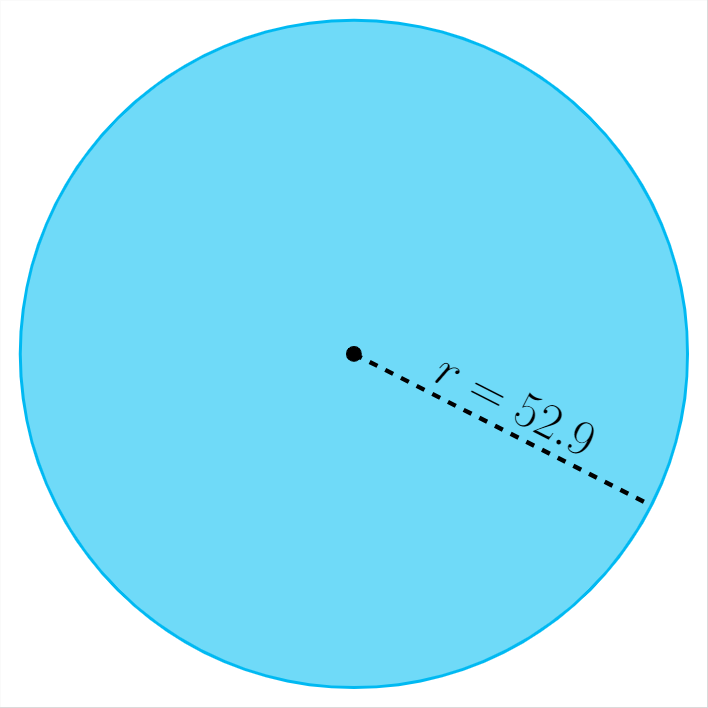
\includegraphics[width=0.7\linewidth]{mex_0004.png}

                        Perímetro: \fillin[$x$ u][0in] \qquad \qquad Área: \fillin[$x$ u$^2$][0in]

                        \begin{solutionbox}{4cm}
                        \end{solutionbox}

                        \part 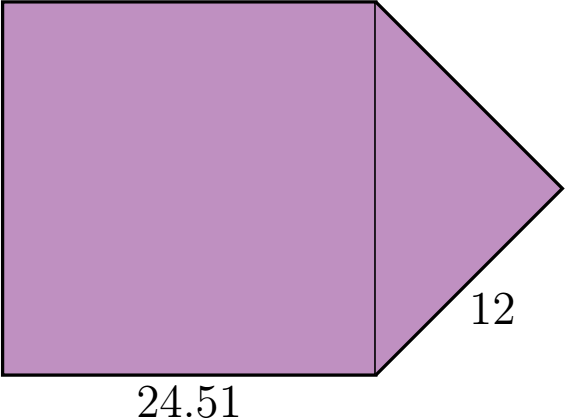
\includegraphics[width=0.7\linewidth]{mex_0014.png}

                        Perímetro: \fillin[$x$ u][0in] \qquad \qquad Área: \fillin[$x$ u$^2$][0in]

                        \begin{solutionbox}{4cm}
                        \end{solutionbox}
                  \end{parts}
            \end{multicols}
      }

      \question[6]{Selecciona la respuesta correcta:
            \begin{multicols}{2}
                  \begin{parts}
                        \part El punto A$(1,0)$, ¿está ubicado sobre el eje $x$?

                        \begin{oneparcheckboxes}
                              \CorrectChoice Verdadero
                              \choice Falso
                        \end{oneparcheckboxes}

                        \part El punto A$(2,0)$, ¿está ubicado sobre el eje $y$?

                        \begin{oneparcheckboxes}
                              \choice Verdadero
                              \CorrectChoice Falso
                        \end{oneparcheckboxes}

                        \part El punto A$(0,-5.9)$, ¿está ubicado sobre el eje $x$?

                        \begin{oneparcheckboxes}
                              \choice Verdadero
                              \CorrectChoice Falso
                        \end{oneparcheckboxes}

                        \part El punto A$(0,8.24)$, ¿está ubicado sobre el eje $y$?

                        \begin{oneparcheckboxes}
                              \CorrectChoice Verdadero
                              \choice Falso
                        \end{oneparcheckboxes}

                        \part El punto A$(-1.5,0)$, ¿está ubicado sobre el eje $x$?

                        \begin{oneparcheckboxes}
                              \CorrectChoice Verdadero
                              \choice Falso
                        \end{oneparcheckboxes}

                        \part El punto A$(0,-10)$, ¿está ubicado sobre el eje $x$?

                        \begin{oneparcheckboxes}
                              \choice Verdadero
                              \CorrectChoice Falso
                        \end{oneparcheckboxes}

                  \end{parts}
            \end{multicols}
      }

      % \subsection*{Resolución de problemas}
      % \question[4]{Resuelve los siguientes problemas:
      %       \begin{multicols}{2}
      %             \begin{parts}\footnotesize%
      %                   \part Calcula la altura de un prisma que tiene como área de la base 6 m$^2$ y 66 m$^3$ de capacidad.

      %                   \begin{solutionbox}{1cm}
      %                   \end{solutionbox}



      %                   \part ¿Cuál es el perímetro de un campo de fútbol que mide 95.12 metros de largo y 45.27 metros de ancho?

      %                   \begin{solutionbox}{1cm}
      %                   \end{solutionbox}
      %             \end{parts}
      %       \end{multicols}
      % }

      % \subsection*{Área lateral, Área total y Volumen}
      \question[10]{Calcula el volumen, el área lateral y el área total de las siguientes figuras:

            \begin{multicols}{2}
                  \begin{parts}
                        \part 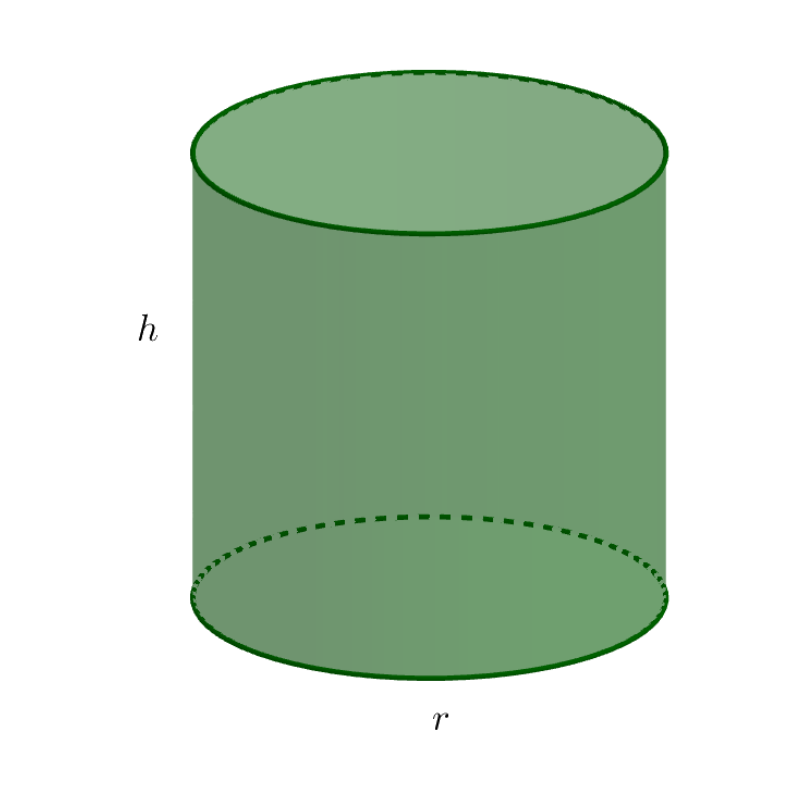
\includegraphics[width=0.8\linewidth]{mex_0024.png}

                        Cilindro con altura $h=17$ cm y un radio $r=4$ cm.\\

                        Área Lateral: \fillin[$x$ u][0in]

                        \begin{solutionbox}{2cm}
                        \end{solutionbox}

                        Área Total: \fillin[$x$ u$^2$][0in]

                        \begin{solutionbox}{2cm}
                        \end{solutionbox}

                        Volumen: \fillin[$x$ u$^3$][0in]

                        \begin{solutionbox}{2cm}
                        \end{solutionbox}

                        \part 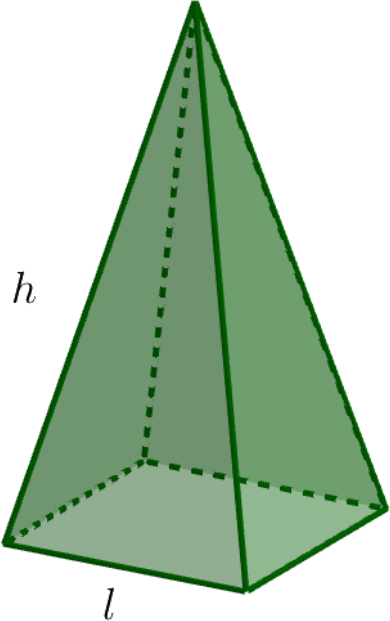
\includegraphics[width=0.8\linewidth]{mex_0029.png}

                        Pirámide cuyos lados "l" de la base miden 16 cm y la altura "h" mide 27 cm.\\

                        Área Lateral: \fillin[$x$ u][0in]

                        \begin{solutionbox}{2cm}
                        \end{solutionbox}

                        Área Total: \fillin[$x$ u$^2$][0in]

                        \begin{solutionbox}{2cm}
                        \end{solutionbox}

                        Volumen: \fillin[$x$ u$^3$][0in]

                        \begin{solutionbox}{2cm}
                        \end{solutionbox}

                  \end{parts}
            \end{multicols}
      }





      \question[10]{Escribe la ecuación de las recta para dada uno de los siguientes incisos:

            \begin{multicols}{2}
                  \begin{parts}
                        \part Escribe la ecuación de la recta que pasa por los puntos A(1,6) y B(2,1)

                        \begin{solutionbox}{2.5cm}
                        \end{solutionbox}

                        \part Escribe la ecuación de la recta que pasa por los puntosA(-2,3) y B(1,0)

                        \begin{solutionbox}{2.5cm}
                        \end{solutionbox}
                  \end{parts}
            \end{multicols}
      }

      % \subsection*{Cuadrantes en el plano cartesiano}

      % \subsection*{Pendiente y ordenada}
      % \question[5]{Identifica la pendiente y ordenada de las siguientes rectas:
      %       \begin{parts}
      %             \begin{multicols}{3}
      %                   \part $y=-2x+1$ \\[1em]
      %                   Pendiente = \fillin[$-2$][0in] \\  Ordenada = \fillin[$1$][0in]

      %                   \part $y=\dfrac{1}{2}x-3$ \\[1em]
      %                   Pendiente = \fillin[$\dfrac{1}{2}$][0in]  \\ Ordenada = \fillin[$-3$][0in]

      %                   \part $y=-3x+3$ \\[1em]
      %                   Pendiente = \fillin[$-3$][0in] \\  Ordenada = \fillin[$3$][0in]
      %             \end{multicols}

      %             \begin{multicols}{2}
      %                   \part 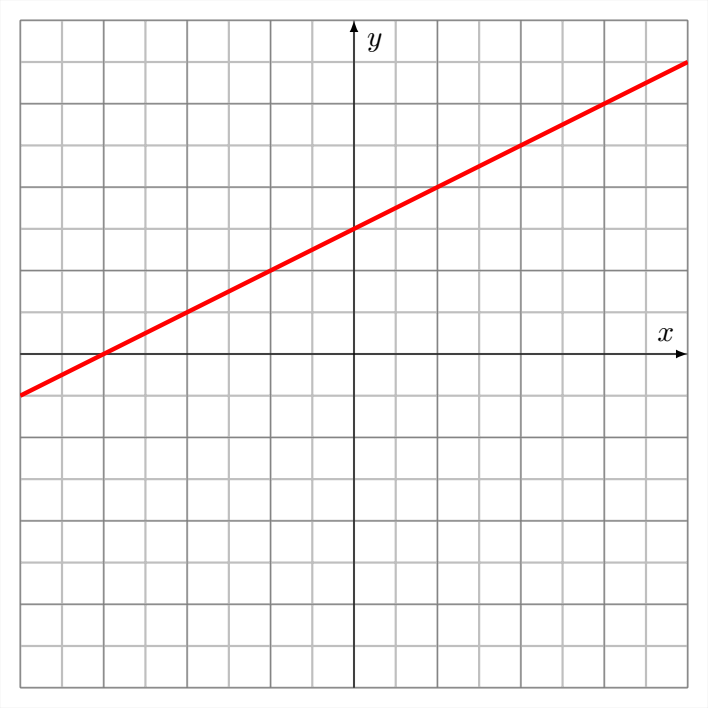
\includegraphics[width=0.8\linewidth]{mex_0047.png}\\
      %                   Pendiente = \fillin[$-2$][0in] \qquad \qquad Ordenada = \fillin[$1$][0in]

      %                   \part 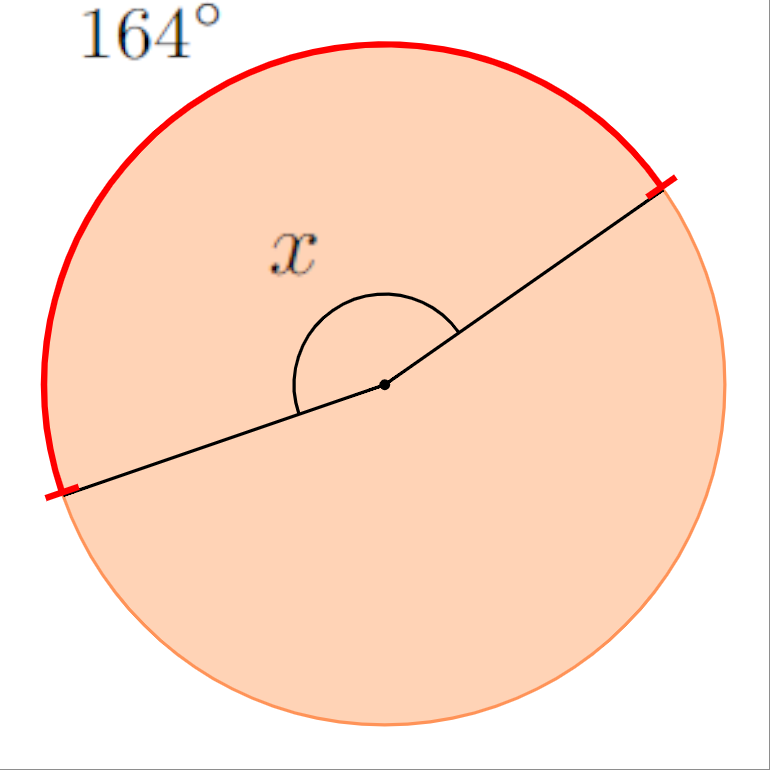
\includegraphics[width=0.8\linewidth]{mex_0051.png}\\
      %                   Pendiente = \fillin[$-2$][0in]  \qquad \qquad Ordenada = \fillin[$1$][0in]
      %             \end{multicols}

      %       \end{parts}
      % }



      % \subsection*{Pendiente dados dos puntos}
      % \question[7]{Calcula la pendiente en cada uno de los siguientes incisos:
      %       \begin{multicols}{2}

      %             \begin{parts}
      %                   \part Calcula la pendiente de la recta que pasa por los puntos A(0,-3) y B(5,1).   \\[1em]
      %                   $m=$ \fillin[$\dfrac{4}{5}$][0in]
      %                   \part Calcula la pendiente de la recta que pasa por los puntos A(-8,6) y B(-3,8).  \\[1em]
      %                   $m=$ \fillin[$\dfrac{2}{5}$][0in]
      %                   \part Calcula la pendiente de la recta que pasa por los puntos A(1,1) y B(5,-3).   \\[1em]
      %                   $m=$ \fillin[$-1$][0in]
      %                   \part Calcula la pendiente de la recta que pasa por los puntos A(-7,-3) y B(6,10). \\[1em]
      %                   $m=$ \fillin[$1$][0in]
      %                   \part Calcula la pendiente de la recta que pasa por los puntos A(-7,-3) y B(-5,7). \\[1em]
      %                   $m=$ \fillin[$5$][0in]

      %                   \part Calcula la pendiente de la siguiente recta:\\
      %                   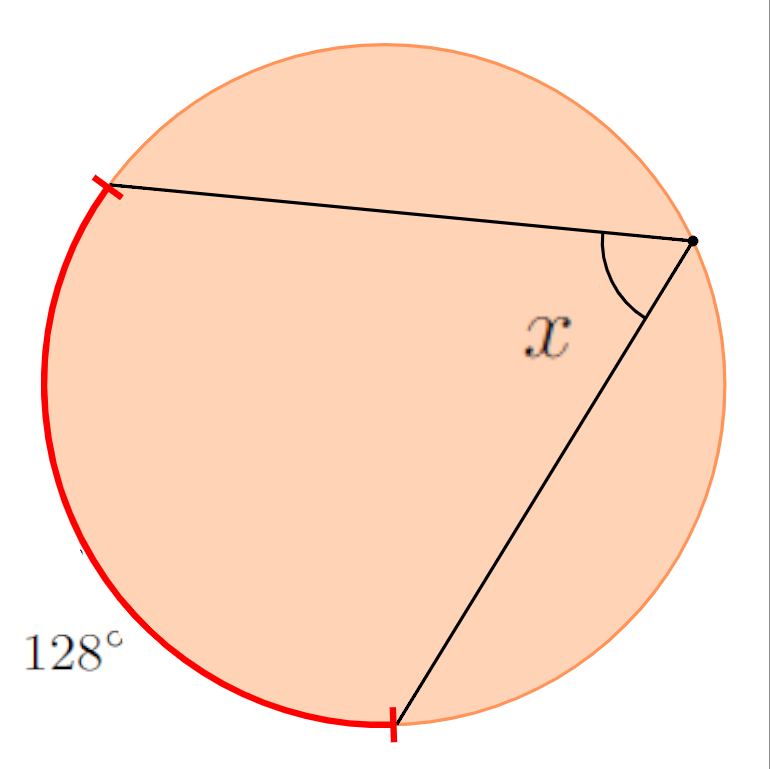
\includegraphics[width=0.8\linewidth]{mex_0050.png} $m=$ \fillin[$-1$][0in]

      %                   \part Calcula la pendiente de la siguiente recta:\\
      %                   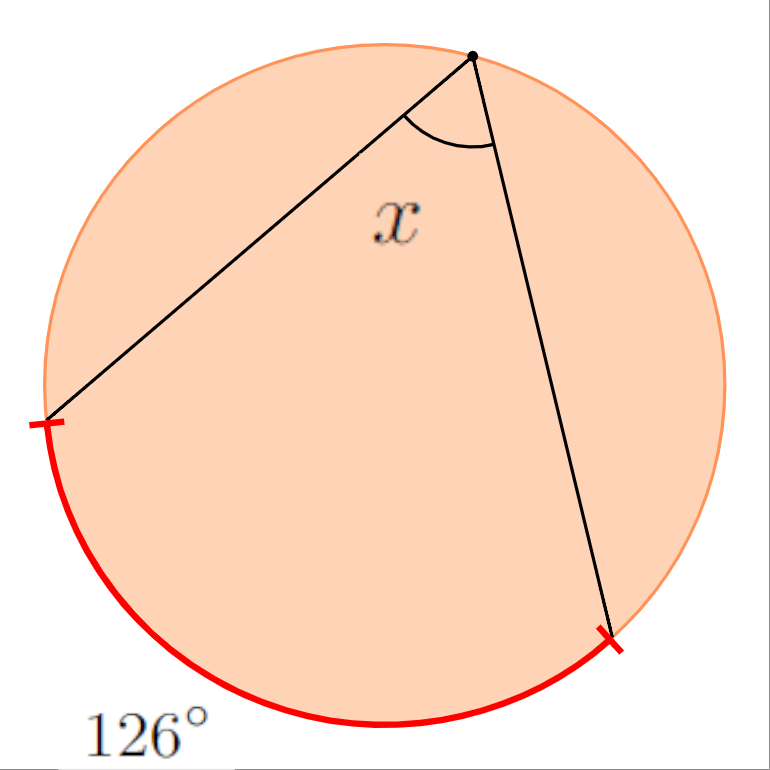
\includegraphics[width=0.8\linewidth]{mex_0048.png} $m=$ \fillin[$\dfrac{4}{5}$][0in]
      %             \end{parts}
      %       \end{multicols}
      % }

      % \section*{Ecuación lineal}

      % \subsection*{Ecuaciones lineales}
      \question[10]{Resuelve las siguientes ecuaciones lineales
            \begin{multicols}{2}
                  \begin{parts}
                        % \part $2x=-30$         \fillin[$x=-15$][0in]            \\
                        % \part $x-23=-36$       \fillin[$x=-13$][0in]            \\
                        % \part $-4x=-6$         \fillin[$x=\dfrac{3}{2}$][0in]   \\
                        % \part $6x=-36$         \fillin[$x=-6$][0in]             \\
                        \part $\dfrac{1}{2}x-\dfrac{1}{4}x=\dfrac{1}{8}$

                        \begin{solutionbox}{3cm}
                        \end{solutionbox}

                        % \part $12x-36=-60$     \fillin[$x=-2$][0in]           \\
                        \part $-4x+1=2x+7$     \fillin[$x=-1$][0in]

                        %\part $9x-8=5x+4$      \fillin[$x=3$][0in]

                        \begin{solutionbox}{3cm}
                        \end{solutionbox}
                        % \part $5(-3x+5)=20$    \fillin[$x=\dfrac{1}{3}$][0in] \\

                        % \part $32x+24=5(2x-4)$ \fillin[$x=-2$][0in]

                        % \begin{solutionbox}{1.5cm}
                        % \end{solutionbox}
                  \end{parts}
            \end{multicols}
      }

      % \subsection*{Lenguaje algebraico}
      \question[2]{Escribe la expresión algebraica correcta para los siguientes enunciados
            \begin{multicols}{2}
                  \begin{parts}
                        \part El cubo de un número cualquiera aumentado en 10.

                        \begin{solutionbox}{1cm}
                              $x^3+10$
                        \end{solutionbox}

                        \part El cuadrado de la suma de dos números cualquiera.

                        \begin{solutionbox}{1cm}
                              $(x+y)^2$
                        \end{solutionbox}

                        % \part El recíproco de un número cualquiera.

                        % \begin{solutionbox}{1cm}
                        %       $\dfrac{1}{x}$
                        % \end{solutionbox}



                        % \part La mitad del cubo de la suma de dos números cualquiera.

                        % \begin{solutionbox}{1cm}
                        %       $\dfrac{1}{2}(x+y)^3$
                        % \end{solutionbox}


                  \end{parts}
            \end{multicols}
      }


      % \subsection*{Resolución de problemas}
      \question[5]{Resuelve los siguientes problemas de ecuaciones lineales
            \begin{parts}
                  % \part La suma de tres números consecutivos es 195. Halla estos números
                  % \begin{solutionbox}{2cm}
                  % \end{solutionbox}
                  \part La suma de dos números es 215 y el mayor excede al menor en 31 unidades. ¿Cuáles son estos dos números?

                  \begin{solutionbox}{1.5cm}
                  \end{solutionbox}
            \end{parts}

      }

      % \subsection*{Ecuaciones lineales con fracciones}
      % \question[10]{Resuelve las siguientes ecuaciones lineales con fracciones

      %       \begin{multicols}{2}
      %             \begin{parts}
      %                   \part $\dfrac{1}{2}x-\dfrac{1}{4}x=\dfrac{5}{6}$

      %                   \begin{solutionbox}{1.5cm}
      %                   \end{solutionbox}

      %                   \part $-\dfrac{x}{6}=\dfrac{7}{54}$
      %                   \begin{solutionbox}{1.5cm}
      %                   \end{solutionbox}

      %             \end{parts}
      %       \end{multicols}

      % }



      % \section*{Sistemas de ecuaciones}
      \setlength{\columnsep}{1cm}
      \begin{multicols}{2}
            \question[5]{Utilizando el m\'etodo de tu preferencia, encuentra el valor de $x$ y $y$ para
                  el siguiente sistema de ecuaciones lineales:


                  \begin{eqnarray}
                        13x-6y & = & 22 \nonumber\\
                        x & = & y+6 \nonumber
                  \end{eqnarray}

                  \begin{solutionbox}{6cm}
                  \end{solutionbox}

            }

            \question[5]{Resuelve el siguiente sistema de ecuaciones lineales con fracciones:
                  \begin{align*}
                        12x + 5y                      & = -6  \\
                        \dfrac{5}{3}x - \dfrac{7}{6}y & = -12
                  \end{align*}
                  \begin{solutionbox}{6cm}
                  \end{solutionbox}
            }

      \end{multicols}

      \question[15]{Numera correctamente los pasos para resolver un sistema de dos ecuaciones con dos inc\'ognitas por los m'etodos a continuaci\'on:
            \begin{choices}


                  \choice M\'etodo de suma-resta:
                  \begin{itemize}
                        \item[\rule{1cm}{0.2mm}] Sumar o restar las ecuaciones para eliminar una de las inc\'ognitas.
                        \item[\rule{1cm}{0.2mm}] Multiplicar una o ambas ecuaciones por los n\'umeros necesarios para realizar la eliminaci\'on bajo la suma o resta.
                        \item[\rule{1cm}{0.2mm}] Resolver la ecuaci\'on resultante.
                        \item[\rule{1cm}{0.2mm}] Sustituir los valores en las ecuaciones originales para comprobar que son la soluci\'on.
                        \item[\rule{1cm}{0.2mm}] Sustituir el valor obtenido en una de las ecuaciones iniciales y resolverla.
                  \end{itemize}

                  \choice M\'etodo de sustitución:
                  \begin{itemize}
                        \item[\rule{1cm}{0.2mm}] Resolver la ecuaci\'on resultante.
                        \item[\rule{1cm}{0.2mm}] Despejar una inc\'ognita en una de las ecuaciones.
                        \item[\rule{1cm}{0.2mm}] Sustituir la expresi\'on de esta inc\'ognita en la otra ecuaci\'on para obtener una ecuaci\'on con una sola inc\'ognita.
                        \item[\rule{1cm}{0.2mm}] Sustituir el valor obtenido en la ecuaci\'on en la que aparec\'ia la inc\'ognita despejada.
                        \item[\rule{1cm}{0.2mm}] Sustituir los valores en las ecuaciones originales para comprobar que son la soluci\'on.
                  \end{itemize}

                  \choice M\'etodo de igualaci\'on:
                  \begin{itemize}
                        \item[\rule{1cm}{0.2mm}] Resolver la ecuaci\'on resultante.
                        \item[\rule{1cm}{0.2mm}] Igualar las expresiones para obtener una ecuaci\'on con una inc\'ognita.
                        \item[\rule{1cm}{0.2mm}] Despejar la misma inc\'ognita en ambas ecuaciones.
                        \item[\rule{1cm}{0.2mm}] Sustituir los valores en las ecuaciones originales para comprobar que son la soluci\'on.
                        \item[\rule{1cm}{0.2mm}] Sustituir el valor obtenido en cualquiera de las dos expresiones en las que aparec\'ia despejada la otra inc\'ognita.
                  \end{itemize}
            \end{choices}
      }

      \question[10]{Resuelve el siguiente sistema de ecuaciones lineales:

            \begin{align*}
                  x + 2y +3z  & = 12 \\
                  x - 3y +4z  & = 27 \\
                  -x +  y +2z & = 7
            \end{align*}

            \begin{solutionbox}{8cm}
            \end{solutionbox}
      }
      % \subsection*{Sistema de ecuaciones con fracciones}

\end{questions}
\end{document}